\documentclass{beamer}
\usepackage{hyperref}
\usepackage[T1]{fontenc}
\usepackage{bm}

% other packages
\usepackage{latexsym,amsmath,xcolor,multicol,booktabs,calligra}
\usepackage{graphicx,pstricks,listings,stackengine}

\author{Stats Group}
\title{Final Report: HDP Model}
\institute{Department of Statistics, The University of Chicago}
\date{2023/05/25}
\usepackage{Style}

% defs
\def\cmd#1{\texttt{\color{red}\footnotesize $\backslash$#1}}
\def\env#1{\texttt{\color{blue}\footnotesize #1}}
\definecolor{deepblue}{rgb}{0,0,0.5}
\definecolor{deepred}{rgb}{0.6,0,0}
\definecolor{deepgreen}{rgb}{0,0.5,0}
\definecolor{halfgray}{gray}{0.55}

\lstset{
    basicstyle=\ttfamily\small,
    keywordstyle=\bfseries\color{deepblue},
    emphstyle=\ttfamily\color{deepred},
    stringstyle=\color{deepgreen},
    numbers=left,
    numberstyle=\small\color{halfgray},
    rulesepcolor=\color{red!20!green!20!blue!20},
    frame=shadowbox,
}


\begin{document}

\begin{frame}
    \titlepage
    \begin{figure}[htpb]
        \begin{center}
            
\includegraphics[width=0.25\linewidth]{pic/UChicago_Seal_2Color_MaroonBorder_WhiteFill_CMYK.eps}
        \end{center}
    \end{figure}
\end{frame}

\begin{frame}
    \tableofcontents[sectionstyle=show,subsectionstyle=show,subsubsectionstyle=show]
\end{frame}


\section{Literature Review}

\subsection{\small{Slice Sampler for Mixture Models (Walker, 2007; Kalli et al., 2011)}}
\begin{frame}
    \frametitle{Sampling the Dirichlet Mixture Model with Slices, Walker, 2007}
    \begin{itemize}
        \item In this article, Walker introduce a new method for sampling the mixture of Dirichlet process (MDP) model, a complex task due to the countable infiniteness of the discrete masses from the random distribution functions chosen from the Dirichlet process prior.
        \item Ishwaran and James (2001) recently devised a Gibbs sampling scheme that incorporates more general stick-breaking priors, serving as a direct extension of Escobar's (1988) methodology.
    \end{itemize}
    
\end{frame}

\begin{frame}
    \frametitle{The Dirichlet Process Model}

    The Mixed Dirichlet Process (MDP) model is founded on the concept of creating continuous random distribution functions, as initially proposed by Lo in 1984. The random distribution function selected from a Dirichlet process is almost certain to be discrete, as posited by Blackwell in 1973. Therefore, we turn our attention to the random density function.
    \begin{equation*}
    f_p(y) = \int N(y|\theta)dP(\theta)
    \end{equation*}
    $N(y|\theta)$ denotes a conditional density function, which will typically be a normal distribution with parameters $\theta$. Therefore, in the normal case $\theta = (\mu, \sigma^2)$

\end{frame}

\begin{frame}
    \frametitle{The Dirichlet Process Model}
    Given the form for P, we can write

    \begin{equation*}
    f_{w,\theta}(y) = \sum_j w_j N(y|\theta_j)
    \end{equation*} 
    Via Gibbs sampling ideas, our attempt to estimate the model is to introduce a latent variable $\mu$ such that the joint density of (y,u) given $(\omega, \theta)$ is given by 
    \begin{equation*}
    f_{\omega,\theta}(y,u)= \sum_j \textbf{1} (u < \omega_j)N(y|\theta_j)
    \end{equation*}
    The joint distribution exists and we can write
    
    \begin{equation*}
    f_{\omega, \theta}(y,u) = \sum_{j=1}^{\infty}\omega U(u|0,\omega_j)N(y|\theta_j)
    \end{equation*}

\end{frame}

\begin{frame}
    \frametitle{The Dirichlet Process Model}
    We can get the marginal density for u is given by
    \begin{equation*}
    f_\omega(u)=\sum_{j=1}^{\infty}\omega_j U(u|0,\omega_j) = \sum_{j=1}^{\infty}\textbf{1}(u<\omega_j)
    \end{equation*}
    let $A_\omega(u) = {j:\omega_j>u}$
    then we can get
    \begin{equation*}
    f_{\omega, \theta}(y, u) = \sum_{j\in A_\omega(u)} N(y|\theta_j)
    \end{equation*}
    It is clear that $A_\omega(u)$ is a finite set for all u>0. The conditional density of y given u is
    \begin{equation*}
    f_{\omega, \theta}(y|u)=\frac{1}{f_\omega(u)}\sum_{j \in A_\omega(u)} N(y|\theta_j)
    \end{equation*}
    
\end{frame}

\begin{frame}
    \frametitle{The Dirichlet Process Model}
    Here, we move from an infinite sum to a finite sum, which makes a lot of difference when sampling involved.
    \newline
    Thus, given u, we have a finite mixture model with equal to $1/f_\omega(u)$. 
    \newline
    We can introduce a further indicator latent variable which will identify the component of the mixture from which y is to be taken.
    Joint density:
    \begin{equation*}
    f_{\omega, \theta}(y,\delta=k, u) = N(y|\theta_k)\textbf{1}(k\in A(u))
    \end{equation*}
    The complete data likelihood based on a sample of size n:
    \begin{equation*}
    l_{\omega, \theta}({y_i, u_i, \delta_i = k_i}_{i=1}^n)=\prod_{i=1}^n N(y_i|\theta_{k_i})\textbf{1}(u_i<\omega_{k_i})
    \end{equation*}
\end{frame}




\begin{frame}
    \frametitle{Slice Sampling Mixture Models, Kalli, 2011}
    \begin{itemize}
        \item In this article, Kalli et.al (2011) proposed a modified slice sampler called slice efficient sampler for inference problems of Dirichlet process mixture models. While preserving the property of reducing infinite number of components to finite number, slice efficient sampler is able to control the updating process of  auxiliary variables so that the MCMC sampling process is smooth.
        \item The authors extended the idea of slice sampler to normalized weights priors for mixture models and performed two numerical experiments to demonstrate the effeteness of slice sampler.
    \end{itemize}
\end{frame}


\begin{frame}
    \frametitle{Slice Sampling Mixture Models, Kalli, 2011}
        Slice efficient sampler: by introducing $\zeta_i$, $i=1,2,3,4,...$, a positive decreasing deterministic sequence and $d$, a latent variable indicating which finite number of components can produce the observed data $y$. $d$ together with $u$, where $u$ here is the auxiliary variable, reduce the infinite number of mixture of components to finite components so that MCMC algorithms are smooth. The construction is followed:\\
        $$
        f_{v,\mu,\sigma^2}(y,u, d) = \zeta^{-1}_d \textbf{1}(u < \zeta_{d}) w_d N(y;u_d, \sigma^2_d)
        $$\\
        The joint posterior likelihood is then:
        $$
        \prod_{i=1}^n \zeta^{-1}_{d_i} \textbf{1}(u < \zeta_{d_i}) w_{d_i} N(y;u_{d_i}, \sigma^2_{d_i})
        $$
\end{frame}

\begin{frame}
    \frametitle{Slice Sampling Mixture Models, Kalli, 2011}
    Notice, here $\zeta_{i}$ is decreasing and is positive, so $\textbf{1}(u < \zeta_{i})$ happens with less chance, while $\frac{w_i}{\zeta_{i}}$ gets bigger so gives more weights to the Gaussian kernel. Thus, the sampling algorithm is followed:
    $$
    \begin{aligned}
    & 1. \pi\left(\mu_{j}, \sigma_{j}^{2} \mid \cdots\right) \propto p_{0}\left(\mu_{j}, \sigma_{j}^{2}\right) \prod_{d_{i}=j} \mathrm{~N}\left(y_{i} ; \mu_{j}, \sigma_{j}^{2}\right) \\
    & 2. \pi\left(v_{j}\right) \propto \mathrm{Be}\left(v_{j} ; a_{j}, b_{j}\right),  a_{j}=1+\sum_{i=1}^{n} \textbf{1}\left(d_{i}=j\right), b_{j}=M+\sum_{i=1}^{n} \textbf{1}\left(d_{i}>j\right) \\
    & 3. \pi\left(u_{i} \mid \cdots\right) \propto \textbf{1}\left(0<u_{i}<\xi_{d_{i}}\right) \\
    & 4. \mathrm{P}\left(d_{i}=k \mid \cdots\right) \propto \textbf{1}\left(k: \xi_{k}>u_{i}\right) w_{k} / \xi_{k} \mathrm{~N}\left(y_{i} ; \mu_{k}, \sigma_{k}^{2}\right)
    \end{aligned}
    $$
\end{frame}



\begin{frame}
    \frametitle{Slice Sampling Mixture Models, Kalli, 2011}
Mixtures based on normalized weights prior \\
    \begin{itemize}
    \item Consider $f(y)=\sum_{j=1}^{\infty} w_{j} K\left(y ; \phi_{j}\right)$,  $w_{j}=\lambda_{j} / \Lambda, \Lambda=\sum_{j=1}^{\infty} \lambda_{j}$ and $\phi_{1}, \phi_{2}, \phi_{3}, \ldots$ are iid.
    $\Lambda_{m}=\sum_{j=m+1}^{\infty} \lambda_{j}$ and $\lambda_{j} \sim \pi_{j}\left(\lambda_{j}\right)$
    \item  $\pi_j$ as the authors suggested can be gamma distribution and inverse Gaussian distribution
    \end{itemize}
\end{frame}

\begin{frame}
    \frametitle{Slice Sampling Mixture Models, Kalli, 2011}
    Slice sampler and normalized weights prior 
    \begin{itemize}
    \item joint density: $$f(y, v, u, d)=\exp (-v \Lambda) \textbf{1}\left(u<\xi_{d}\right) \lambda_{d} / \xi_{d} K\left(y ; \phi_{d}\right)$$
    \item let  $v_1, v_2,...,v_{n}$ be $v=\sum_{i=1}^{n} v_{i}$, the likelihood is then $$v^{n-1} \exp (-v \Lambda) \prod_{i=1}^{n} \textbf{1}\left(u_{i}<\xi_{d_{i}}\right) \lambda_{d_{i}} / \xi_{d_{i}} K\left(y_{i} ; \phi_{d_{i}}\right)$$
    \end{itemize}
    Then, the authors provided two algorithms to perform sampling:\\
    (1) dependent slice-efficient sampler and $\xi_{j}=\lambda_{j}$\\
    (2) independent slice-efficient sampler and $\xi_{j}$, $\lambda_{j}$ independent
\end{frame}

\begin{frame}
    \frametitle{Slice Sampling Mixture Models, Kalli, 2011}
        \begin{itemize}
            \item Random hazard function has same posterior as normalized mixture models using slice efficient sampler
            \item The authors compared the efficiency of slice sampler and retrospective sampler, pointing out that slice sampler can save much pre-runnung work and so easier to work.
    
        \end{itemize}
\end{frame}







\subsection{\small{HDP Model (Teh et al., 2004)}}
\begin{frame}
    \frametitle{Main Idea}
    \begin{itemize}
        \item The paper discusses the representation of hierarchical Dirichlet processes using a \textbf{stick-breaking process} and introduces a generalization of the Chinese restaurant process called the \textbf{“Chinese restaurant franchise.”} These representations facilitate the understanding and implementation of hierarchical Dirichlet processes.
    \end{itemize}
\end{frame}
\begin{frame}
    \frametitle{Dirichlet Process}
    \begin{itemize}
        \item Let $(\Theta, B)$ be a measurable space, with $G_0$ a probability measure on the space. Let $\alpha_0$ be a positive real number. For any finite partition $\{A_1,...,A_k\}$ of the sample space, consider the random vector $(G(A_1),...,G(A_k))$ where $G()$ is a random distribution function. If
$$(G(A_1),...,G(A_k))\sim Dirichlet(\alpha_0, G_0(A_1),...,G_0(A_k))$$

where $G_0$ is also a fixed distribution function, then $G \sim DP(\alpha_0,G_0)$ is a Dirichlet process.
    \end{itemize}
\end{frame}
\begin{frame}
    \frametitle{Dirichlet process}
    \begin{itemize}
        \item We have the model
$$\begin{aligned}\theta_{i}|G &\sim G\\
x_{i}|\theta_{i}&\sim F(\theta_{i})\end{aligned}$$
where $F(\theta_{i})$ denotes the distribution of the observation $x_i$ given $\theta_{i}$. The factors $\theta_{i}$ are conditionally independent given $G$, and the observation $x_i$ is conditionally independent of the other observations given the factor $\theta_{i}$. 
    \item When $G$ is distributed according to a Dirichlet process, this model is referred to as a Dirichlet process mixture model.
    \end{itemize}
\end{frame}
\begin{frame}
    \frametitle{Hierarchical Dirichlet processes}
    \begin{itemize}
        \item We have the global random probability measure $G_0$,
$$G_0|\gamma, H\sim DP(\gamma, H)$$
        \item We have conditional random measure $G_j$ follow,
$$G_j|\alpha_0, G_0\sim DP(\alpha_0, G_0)$$
        \item In this model we have three hyper-parameters: baseline probability measure $H$, concentration parameters $\gamma,\alpha_0$
    \end{itemize}
\end{frame}
\begin{frame}
    \frametitle{Hierarchical Dirichlet processes}
    \begin{itemize}
        \item For now, we can have HDP
$$\begin{aligned}\theta_{ji}|G_j &\sim G_j\\
G_j|\alpha_0, G_0&\sim DP(\alpha_0, G_0)\\
G_0|\gamma,H &\sim DP(\gamma,H)\\
x_{ji}|\theta_{ji}&\sim F(\theta_{ji}),\ \text{for each}\ j\ \text{and}\ i
\end{aligned}$$
    \end{itemize}
\end{frame}
\begin{frame}
    \frametitle{Hierarchical Dirichlet processes}
    \begin{figure}[H] 
    \centering
    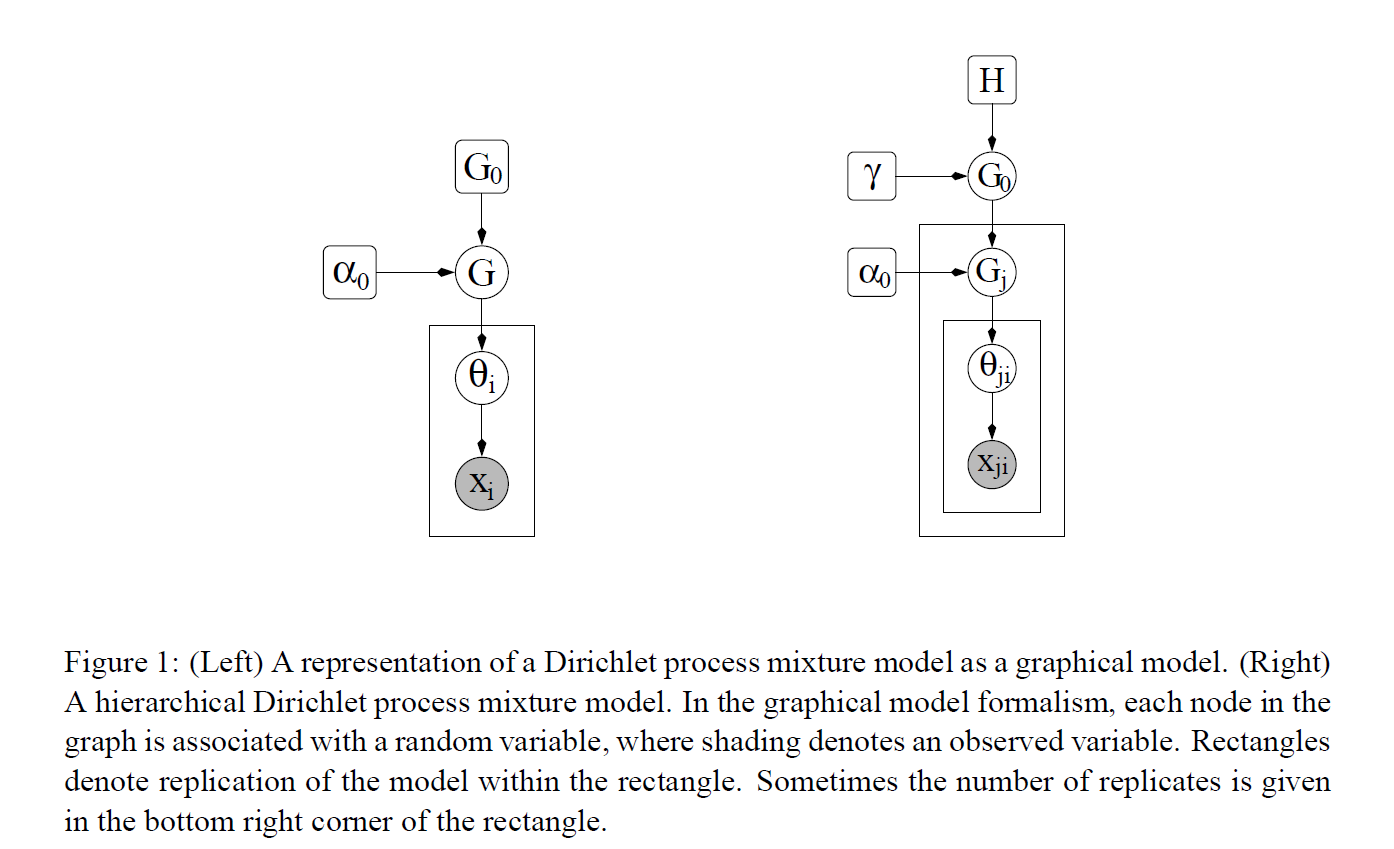
\includegraphics[width=1\textwidth]{pic/2023-05-16 185113.png} 
    \caption{} 
    \label{Fig1} 
    \end{figure}
\end{frame}
\begin{frame}
    \frametitle{Stick-breaking Representation}
    \begin{itemize}
        \item Given that the global measure $G_0$ is distributed as a Dirichlet process, it can be expressed using a stick-breaking representation:
$$G_0=\sum_{k=1}^\infty \beta_k\delta_{\phi_k}\ \ (16)$$
where $\phi_k\sim H$ independently and $\beta = (\beta_k)_{k=1}^\infty \sim \text{GEM}(\gamma)$ are mutually independent. Since $G_0$ has support at the points $\phi = (\phi_k)^\infty_{k=1}$, each $G_j$ necessarily has support at these points as well, and
can thus be written as:
$$G_j=\sum_{k=1}^\infty \pi_{jk}\delta_{\phi_k}\ \ (17)$$
    \end{itemize}
\end{frame}
\begin{frame}
    \frametitle{Stick-breaking Representation}
    \begin{itemize}
        \item Let $\pi_{j} = (\pi_{jk})^\infty_{k=1}$. Note that the weights $\pi_j$ are independent given $\beta$ (since the $G_j$ are independent given $G_0$). We now describe how the weights $\pi_j$ are related to the global weights $\beta$.
        \item Let $(A_1,...,A_r)$ be a measurable partition, and $K_l=\{k:\phi_k \in A_l\},l=1,...,r$ is a finite partition of the positive integers. We have 
$$\begin{aligned}(G_j(A_1),...,G_j(A_r)) &\sim Dir(\alpha_0G_0(A_1),...,\alpha_0G_0(A_r))\\
\Rightarrow (\sum_{k\in K_1}\pi_{jk},...,\sum_{k\in K_r}\pi_{jk})&\sim Dir(\alpha_0\sum_{k\in K_1}\beta_{k},...,\alpha_0\sum_{k\in K_r}\beta_{k})\ \ (18)\end{aligned}$$
    \end{itemize}
\end{frame}
\begin{frame}
    \frametitle{Stick-breaking Representation}
    \begin{itemize}
        \item Then try to derive the explicit relationship of $\beta, \pi_j$. 
$$\begin{aligned}\beta_k'\sim Beta(1,\gamma),\ \ \beta_k=\beta_k'\Pi_{l=1}^{k-1}(1-\beta_l')\ \ (20)\end{aligned}$$
        \item It can be showed that the following stick-breaking construction produces a random probability measure $\pi_j\sim DP(\alpha_0,\beta)$:
$$\begin{aligned}\pi_{jk}'\sim Beta(\alpha_0\beta_k,\alpha_0(1-\sum_{l=1}^k \beta_l)),\ \ \pi_{jk}=\pi_{jk}'\Pi_{l=1}^{k-1}(1-\pi_{jl}')\ \ (21)\end{aligned}$$
    \end{itemize}
\end{frame}
\begin{frame}
    \frametitle{Stick-breaking Representation}
    \begin{itemize}
        \item To derive (21), first notice that for a partition $(\{1,..., k-1\}, \{k\}, \{k+1,k+2,...\})$, (18) gives
$$(\sum_{l=1}^{k-1}\pi_{jl},\pi_{jk},\sum_{l=k+1}^{\infty}\pi_{jl})\sim Dir(\alpha_0\sum_{l=1}^{k-1}\beta_{l},\alpha_0\beta_{k},\alpha_0\sum_{l=k+1}^{\infty}\beta_{l})\ \ (22)$$
        \item Removing the first element, and using standard properties of the Dirichlet distribution that support should be added to 1(Re-normalization Property). Dirichlet Distribution follows the renormalization property. Let $\pi_1,...,\pi_K\sim Dir(\alpha_1,...,\alpha_K)$,
$$\frac{(\pi_2,...,\pi_K)}{\sum_{k=2}^K \pi_k}\sim Dir(\alpha_2,...,\alpha_K)$$
    \end{itemize}
\end{frame}
\begin{frame}
    \frametitle{Stick-breaking Representation}
    \begin{itemize}
        \item So we have
$$\frac{1}{1-\sum_{l=1}^{k-1}\pi_{jl}}(\pi_{jk},\sum_{l=k+1}^{\infty}\pi_{jl})\sim Dir(\alpha_0\beta_{k},\alpha_0\sum_{l=k+1}^{\infty}\beta_{l})\ \ (23)$$
        \item Finally, define $\pi_{jk}'=\frac{\pi_{jk}}{1-\sum_{l=1}^{k-1}\pi_{jl}}$ and notice that $1-\sum_{l=1}^k \beta_l=\sum_{l=k+1}^{\infty}\beta_{l}$ to obtain (21)
$$\begin{aligned}(\pi_{jk}',1-\pi_{jk}')\sim Dir(\alpha_0\beta_{k},\alpha_0(1-\sum_{l=1}^k \beta_l))\\
\Rightarrow \pi_{jk}'\sim Beta(\alpha_0\beta_k,\alpha_0(1-\sum_{l=1}^k \beta_l))\end{aligned}$$
    \end{itemize}
\end{frame}
\begin{frame}
    \frametitle{Chinese Restaurant Franchise (CRF) Process}
    \begin{itemize}
        \item Different from original Chinese Restaurant Process, We have a restaurant franchise with a shared menu across the restaurants. 
        \item At each table of each restaurant one dish is ordered from the menu by the first customer who sits there, and it is shared among all customers who sit at that table. Multiple tables in multiple restaurants can serve the same dish.
    \end{itemize}
\end{frame}
\begin{frame}
    \frametitle{Chinese Restaurant Franchise (CRF) Process}
    Process assumes $j = 1,...,J$ Chinese restaurants:
    \begin{itemize}
        \item with infinite tables in each restaurant;
        \item all share the same menu;
        \item 1st customer to a new table orders a plate for the table;
        \item multiple tables in multiple restaurants can serve the same plate.
    \end{itemize}
    Each customer $i$ entering a restaurant $j$ does the following:
    \begin{itemize}
        \item Chooses a table to sit proportion to the number of customers already at that table.
        \item If sits in a new table, then order a plate from the menu proportion to the popularity of the plate across all restaurants.
    \end{itemize}
\end{frame}



\section{Repeat and Research}
\subsection{\small{Repeat: Chinese Restaurant Franchise Sampling Method}}
	\begin{frame}
		\frametitle{The Chinese Restaurant Franchise}
		\begin{itemize}
			\item The Chinese restaurant process is extended to allow multiple restaurants to share a set of dishes.
		\end{itemize}
		\begin{figure}[H]
			\centering
			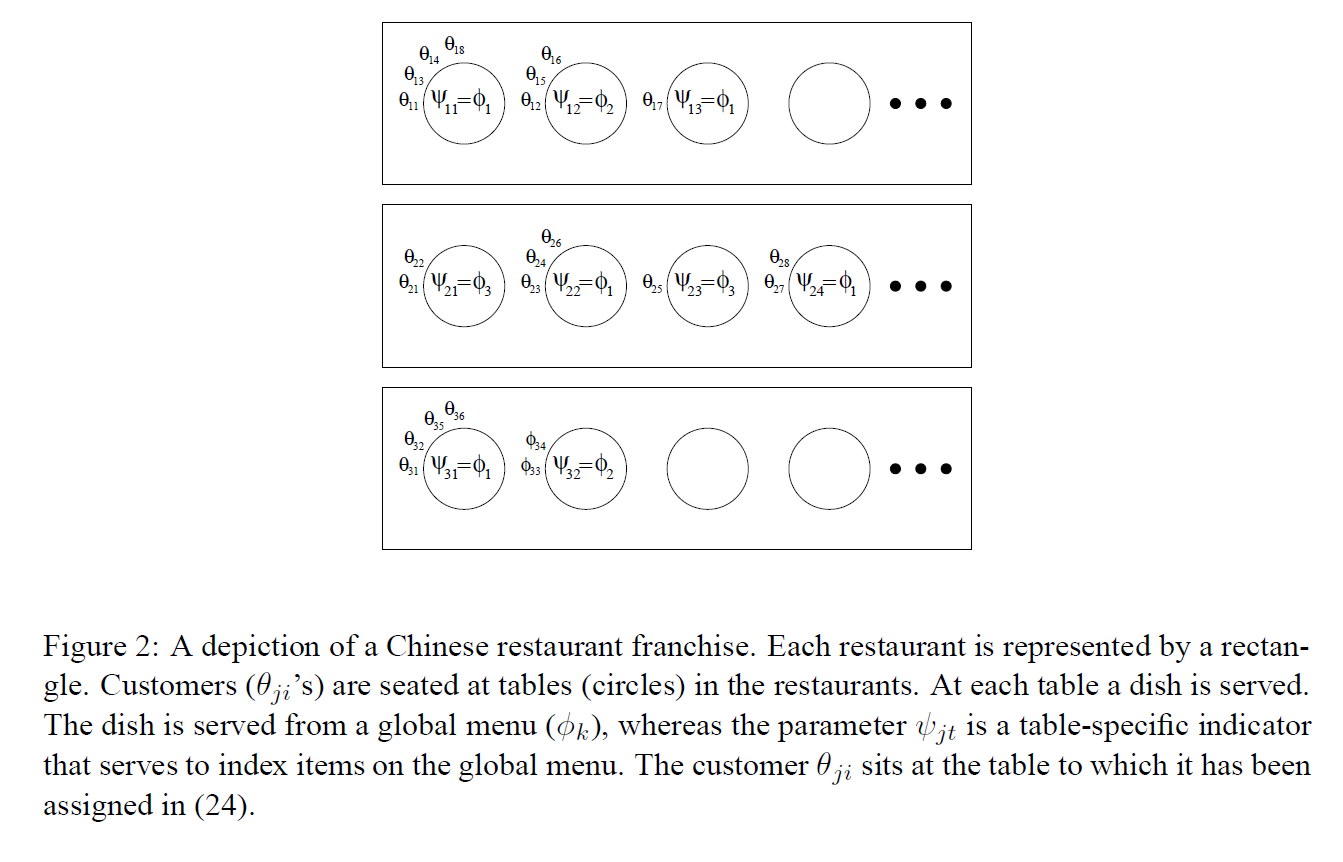
\includegraphics[width=9cm]{pic/2023-05-16 185245.png}
		\end{figure}
	\end{frame}
	\begin{frame}
		\frametitle{The Chinese Restaurant Franchise Notations}
		\begin{itemize}
			\item $\theta_{ji}$: customers; $\phi_k$: a global menu
			\item $x_{ji}$: the observed data, each one is a draw from a distribution $F(\theta_{ji})$
			\item $\psi_{jt}$: the dish served at table $t$ in restaurant $j$
			\item $t_{ji}$: the index of the $\psi_{jt}$ associated with $\theta_{ji}$
			\item  $k_{jt}$: the index of $\phi_k$ associated with $\psi_{jt}$
			\item We also maintain counts of customers and counts of tables \\ $n_{jtk}$: the number of customers in restaurant $j$ at table $t$ eating dish $k$ \\ $m_{jk}$: the number of tables in restaurant $j$ serving dish $k$
		\end{itemize}
	\end{frame}
	\begin{frame}
		\frametitle{The Chinese Restaurant Franchise}
		\begin{equation}
			\theta_{ji} \mid \theta_{j1},\cdots,\theta_{j,i-1},\alpha_0,G_0 \sim \sum_{t=1}^{m_{j\cdot}}\frac{n_{jt\cdot}}{i-1+\alpha_0}\delta_{\psi_{jt}} + \frac{\alpha_0}{i-1+\alpha_0}G_0
		\end{equation}
		\begin{equation}
			\psi_{jt} \mid \psi_{11},\psi_{12},\cdots,\psi_{21},\cdots,\psi_{j,t-1},\gamma,H \sim \sum_{k=1}^{K}\frac{m_{\cdot k}}{m_{\cdot \cdot}+\gamma}\delta_{\phi_{k}} + \frac{\gamma}{m_{\cdot \cdot}+\gamma}H
		\end{equation}
		For each $j$ and $i$, first sample $\theta_{ji}$ using (1). If a new sample from $G_0$ is needed, we use (2) to obtain a new sample $\psi_{jt}$ and set $\theta_{ji}=\psi_{jt}$
	\end{frame}
	\begin{frame}
		\frametitle{Posterior Sampling in the Chinese Restaurant Franchise}
		\begin{itemize}
			\item Rather than dealing with the $\theta_{ji}$'s and $\psi_{jt}$'s directly, we shall sample their index variables $t_{ji}$ and $k_{jt}$ instead
			\item Motivation: the $\theta_{ji}$'s and $\psi_{jt}$'s can be reconstructed from these index variables and the $\phi_k$'s
			\item Advantage: It makes the MCMC sampling scheme more efficient
			\item Notice that the $t_{ji}$ and $k_{jt}$ inherit the exchangeability properties of the $\theta_{ji}$ and $\psi_{jt}$, allowing us to adapt the conditional distributions in $(1)$ and $(2)$ to be expressed in terms of $t_{ji}$ and $k_{jt}$
		\end{itemize}
	\end{frame}
	\begin{frame}
		\frametitle{Sampling t}
		Obtain the conditional posterior for $t_{ji}$ by combining the conditional prior distribution for $t_{ji}$ with the likelihood of generating $x_{ji}$
		\begin{equation*}
			p(x_{ji}=t \mid \boldsymbol{t}^{-ji},t_{ji}=t^{new},\boldsymbol{k}) = \sum_{k=1}^{K}\frac{m_{\cdot k}}{m_{\cdot \cdot}+\gamma}f_k^{-x_{ji}}(x_{ji}) + \frac{\gamma}{m_{\cdot \cdot}+\gamma}f_{k^{new}}^{-x_{ji}}(x_{ji})
		\end{equation*}
		\begin{equation*}
			p(t_{ji}=t \mid \boldsymbol{t}^{-ji},\boldsymbol{k}) \propto
			\begin{cases}
				n_{jt\cdot}^{-ji}f_{k_{jt}}^{-x_{ji}}(x_{ji})& \text{if $t$ previously used,} \\
				\alpha_0p(x_{ji} \mid \boldsymbol{t})^{-ji},t_{ji}=t^{new},\boldsymbol{k})& \text{if $t=t^{new}$.}
			\end{cases}
		\end{equation*}
	\end{frame}
	\begin{frame}
		\frametitle{Sampling t}
		\begin{itemize}
			\item If the sampled value of $t_{ji}$ is $t^{new}$,
			\begin{equation*}
				p(k_{jt^{new}}=k \mid \boldsymbol{t},\boldsymbol{k}^{-jt^{new}}) \propto
				\begin{cases}
					m_{\cdot k}f_k^{-x_{ji}}(x_{ji})& \text{if $k$ previously used,} \\
					\gamma f_{k^{new}}^{-x_{ji}}(x_{ji})& \text{if $k=k^{new}$.}
				\end{cases}
			\end{equation*}
			\item If some table $t$ becomes unoccupied as a result of updating $t_{ji}$, i.e., $n_{jt\cdot}=0$, then the probability that this table will be reoccupied in the future will be zero. Hence, we delete the corresponding $k_{jt}$ from the data structure.
		\end{itemize}
	\end{frame}
	\begin{frame}
		\frametitle{Sampling k}
		\begin{equation*}
			p(k_{jt}=k \mid \boldsymbol{t},\boldsymbol{k}^{-jt}) \propto
			\begin{cases}
				m_{\cdot k}^{-jt}f_k^{-\boldsymbol{x}_{jt}}(\boldsymbol{x}_{jt})& \text{if $k$ previously used,} \\
				\gamma f_{k^{new}}^{-\boldsymbol{x}_{jt}}(\boldsymbol{x}_{jt})& \text{if $k=k^{new}$.}
			\end{cases}
		\end{equation*}
	\end{frame}
 \begin{frame}
		\frametitle{Implementing the CRF Sampling Method}
		\begin{itemize}
			\item Given hyperparameters: $\alpha_0=\gamma=1$
			\item Priors:
			$\phi_k \mid H \sim H=N(0,\frac{1}{\tau_\phi^2})$, $x_{ji} \mid \theta_{ji} \sim F=N(\theta_{ji},\frac{1}{\tau_x^2})$
			where $\tau_\phi=\tau_x=1$ (predetermined, tuned afterwards)
		\end{itemize}
	\end{frame}
	\begin{frame}
		\frametitle{Implementing the CRF Sampling Method}
		Derive $f_k^{-x_{ji}}(x_{ji})$:
		\begin{equation*}
			f_k^{-x_{ji}}(x_{ji})=\frac{\tau_x}{\sqrt{2\pi}}\tau_\pi\sqrt{\frac{\tau_x^2n_{\cdot\cdot k}^{-ij}+\tau_\phi^2}{\tau_x^2(n_{\cdot\cdot k}^{-ij}+1)+\tau_\phi^2}} e^{-\frac{1}{2}[x_{ji}^2+s_1 -s_2]}
		\end{equation*}
		where $s_1=\frac{(\tau_x^2\sum_{j'i'\neq ji,z_{j'i'}=k}x_{j'i'})^2}{\tau_x^2n_{\cdot\cdot k}^{-ji}+\tau_\phi^2}$ and $s_2=\frac{(\tau_x^2\sum_{z_{j'i'}=k}x_{j'i'})^2}{\tau_x^2n_{\cdot\cdot k}^{-ji}+\tau_\phi^2}$
	\end{frame}
	\begin{frame}
		\frametitle{Result: Trace Plots of $t_{ji}$ and $k_{ji}$}
		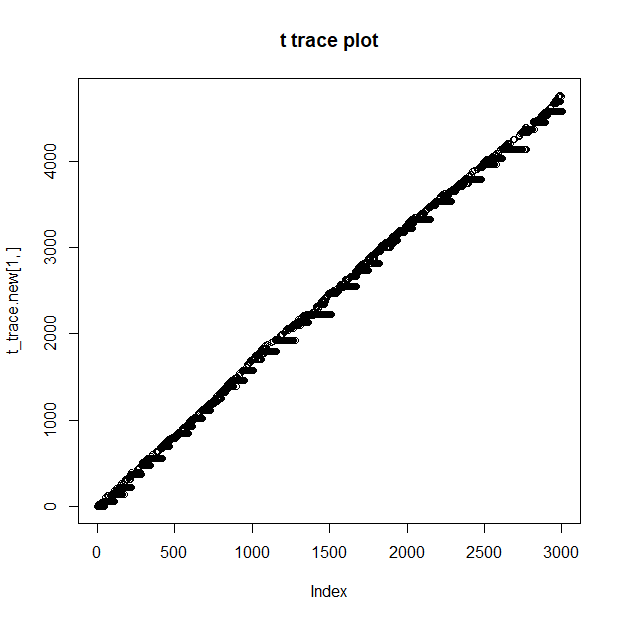
\includegraphics[width=5cm,height=4cm]{pic/image2.png}
		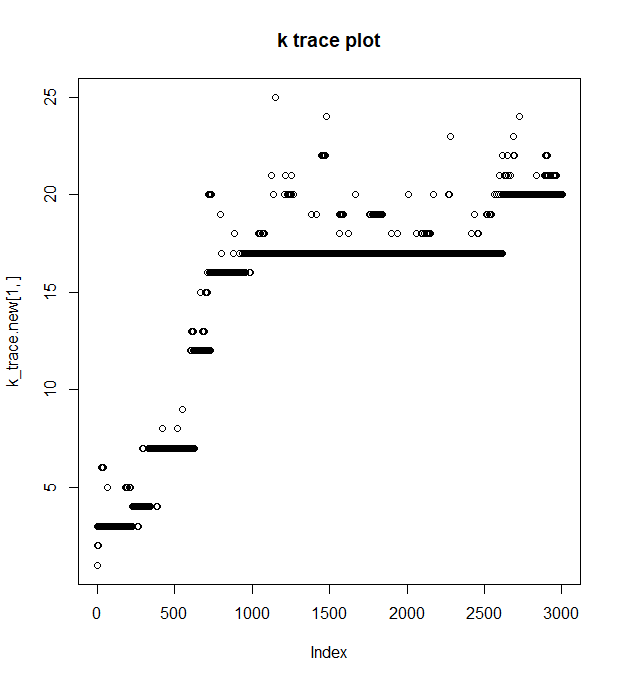
\includegraphics[width=5cm,height=4cm]{pic/image3.png}
	\end{frame}
	\begin{frame}
		\frametitle{Issue: Clustering is not Stable}
		\begin{columns}[t]
			\column{.5\textwidth}
			\centering
			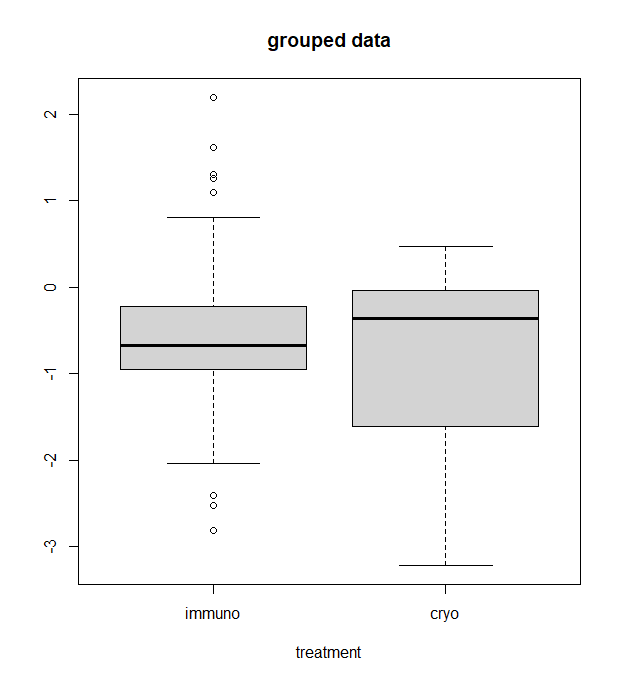
\includegraphics[width=4.5cm,height=3cm]{pic/image4.png}\\
			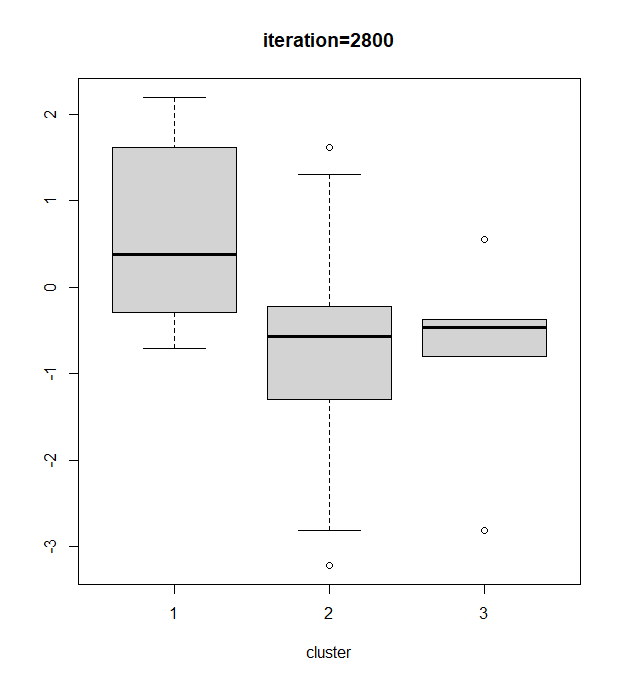
\includegraphics[width=4.5cm,height=3cm]{pic/image5.png}
			\column{.5\textwidth}
			\centering
			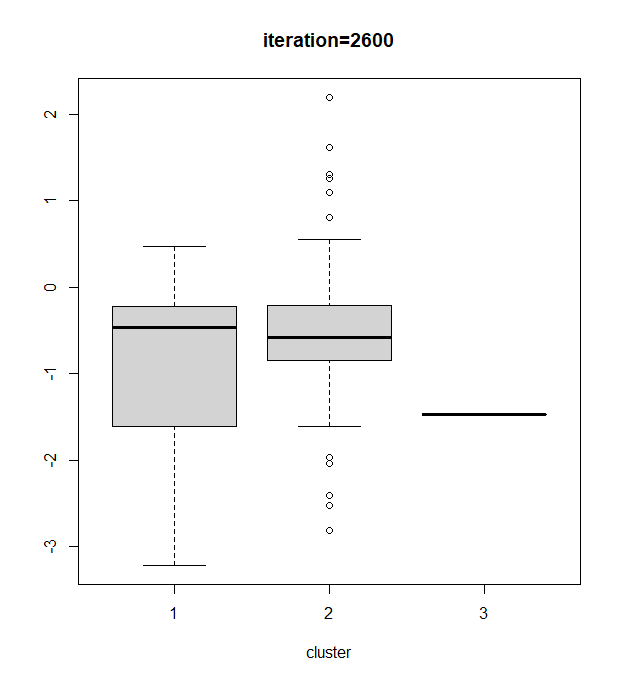
\includegraphics[width=4.5cm,height=3cm]{pic/image6.png}\\
			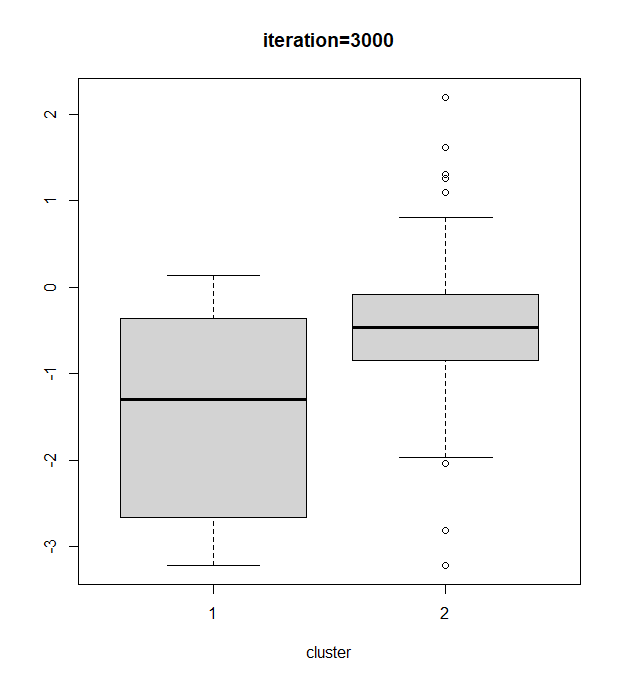
\includegraphics[width=4.5cm,height=3cm]{pic/image7.png}
		\end{columns}
	\end{frame}
	\begin{frame}
		\frametitle{Result: Number of Clusters in Each Iteration}
		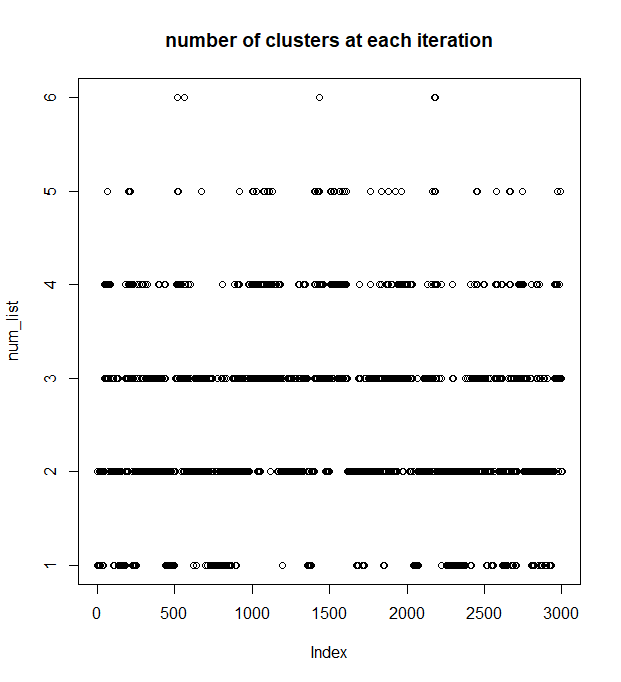
\includegraphics[width=8cm,height=7cm]{pic/image8.png}
	\end{frame}
	\begin{frame}
		\frametitle{Result: Simularity Matrix}
		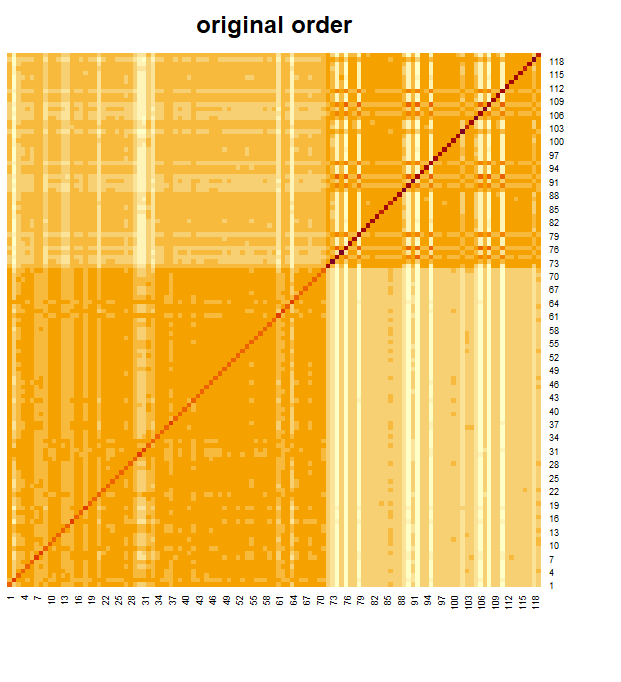
\includegraphics[width=5cm,height=4cm]{pic/image9.png}
		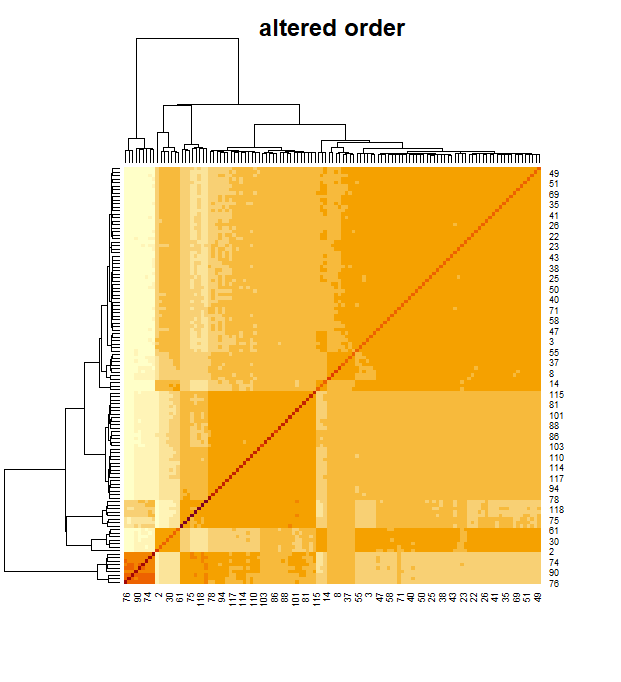
\includegraphics[width=5cm,height=4cm]{pic/image10.png}
	\end{frame}

\subsection{\small{HDP Model with Latent Indicator Variables}}
\begin{frame}
		\frametitle{HDP Model with Latent Indicator Variables (1)}
Our model setting is
\begin{align*}
&y_{ij} \mid \theta_{ij} \sim F(\theta_{ij})
&\theta_{ij} \mid G_j \sim G_j\\
&G_j = \sum_{k = 1}^\infty \pi_{jk}\delta_{\phi_k}
&\pi_{jk} = \pi'_{jk}\prod_{l = 1}^{k-1}(1 - \pi_{jl})\\
&\pi'_{jk} \sim \mathrm{Beta}\biggl(\alpha_0\beta_k, \alpha_0 (1 - \sum_{l=1}^k\beta_l)\biggr)
&\beta_k \sim \beta_k' \prod_{l = 1}^{k-1}(1-\beta'_l)\\
&\beta'_k \sim \mathrm{Beta}(1, \gamma)\\
&\phi_k \sim H \quad (\text{Prior for location } \phi_k)
\end{align*}
\end{frame}


\begin{frame}
\frametitle{HDP Model with Latent Indicator Variables (2)}
\begin{itemize}
\item Now,
\begin{align*}
&F(\cdot) = N(\cdot,\cdot)
&\theta_{ij} = \{\mu_{ij}, \sigma_{ij}^2\}\\
&\phi_{k} = \{\mu_k, \sigma^2_k\}
\end{align*}
\item Then, introduce latent indicator variable $z_{ij}$ indicating which component the observation $ij$ belongs to. In other words,
$$
\theta_{ji} = \phi_{(z_{ji} = k')}
$$
\end{itemize}

\end{frame}


\begin{frame}
\frametitle{HDP Model with Latent Indicator Variables (3)}
Hence, by using $z_{ij}$, we can write the model as
\begin{align*}
&y_{ij} \mid z_{ij},\{\mu_k\}_{k=1}^\infty,\{\sigma^2_k\}_{k=1}^\infty \sim N(\mu_{z_{ij}},\sigma_{z_{ij}})\\
&z_{ij} \mid \{\pi_{jk}\}_{k=1}^\infty \sim \{\pi_{jk}\}_{k=1}^\infty\\
&\pi_{jk} = \pi'_{jk}\prod_{l = 1}^{k-1}(1 - \pi_{jl})\quad \pi'_{jk} \sim \mathrm{Beta}\biggl(\alpha_0\beta_k, \alpha_0 (1 - \sum_{l=1}^k\beta_l)\biggr)\\
&\beta_k \sim \beta_k' \prod_{l = 1}^{k-1}(1-\beta'_l)\quad \beta'_k \sim \mathrm{Beta}(1, \gamma)\\
&\begin{cases}
\mu_k \mid H_\mu \sim H_{\mu}\\
\sigma^2_k \mid H_{\sigma^2} \sim H_{\sigma^2}\\
\end{cases}
\end{align*}

\end{frame}


\subsection{\small{Slice Sampling for HDP}}
\begin{frame}
	\frametitle{A Change of Expression}
	In the initial expression, we have $$ \bm{\beta}|\gamma_0 \sim \text{GEM}(\gamma_0)$$ $$ \bm{\pi}_j|\alpha_0, \bm{\beta} \sim \text{DP}(\alpha_0, \bm{\beta})$$ $$ z_{ij}|\bm{\pi}_j\sim \bm{\pi}_j $$

	However, this expression is not suitable for doing slice sampling, as $\bm{\pi}$ is heavily based on $\bm{\beta}$. Note that $\bm{\pi}$ itself is a DP.
	$$ \bm{\beta}|\gamma \sim \text{GEM}(\gamma_0)$$ $$ \gamma_j|\alpha_0 \sim \text{GEM}(\alpha_0), \gamma_j=(\gamma_{jt}) $$ $$ k_{jt}|\bm{\beta} \sim \bm{\beta}, t=1, 2, 3, ... $$ $$ \bm{\pi}_j = \sum_{t=1}^\infty \gamma_{jt}\delta_{k_{jt}} $$ $$ z_{ji}|\bm{\pi}_j\sim \bm{\pi}_j. $$
\end{frame}

\begin{frame}
	\frametitle{A Change of Expression Cont.}
	This can also be written as the following.
	$$ \bm{\beta}|\gamma \sim \text{GEM}(\gamma_0)$$ $$ \gamma_j|\alpha_0 \sim \text{GEM}(\alpha_0), \gamma_j=(\gamma_{jt}) $$ $$ k_{jt}|\bm{\beta} \sim \bm{\beta}, t=1, 2, 3, ... $$ $$ t_{ij}|\bm{\gamma}_j\sim \bm{\gamma}_j, i=1, 2, ..., n_j $$ $$ z_{ji}|\bm{t_j}, \bm{k}_j = k_{i, t_{ij}}. $$

	We can get the joint density of $\bm{t}, \bm{k}, \bm{\gamma}, \bm{\beta}$, and use this for sampling. (Coding is still in progress...)
	
\end{frame}

\section*{Thanks!}
\begin{frame}
    \begin{center}
        {\Huge\calligra Thanks!}
    \end{center}
\end{frame}

\end{document}